\section{Collisions}\label{sec:collisions}
Continuing from the previous section (\ref{subsec:carriers_sensing}), we now turn our attention to one of the challenges of networking: collisions. 

A collision happens when two or more devices decide to "speak" (transmit data) at the exact same time over the same communication channel. You can imagine why that's problematic. The most common way of dealing with this is to either detect the collision and retransmit the corrupted data or to avoid the collision altogether.

Collisions come in various ca;ibers - partial corruption affects only portions of data, full destruction where entire frames are lost. A particularly interesting case is the hidden terminal problem, where two devices can't detect each other's presence but attempt to communicate with the same destination simultaneously. We'll explore this phenomenon later in the chapter.

Your network interface card (NIC) constantly manages these collision scenarios, implementing detection and recovery mechanisms to maintain reliable communication.
\vfill
% /assets/diagrams/csma/collisions.png
\begin{figure}[h]
    \centering
    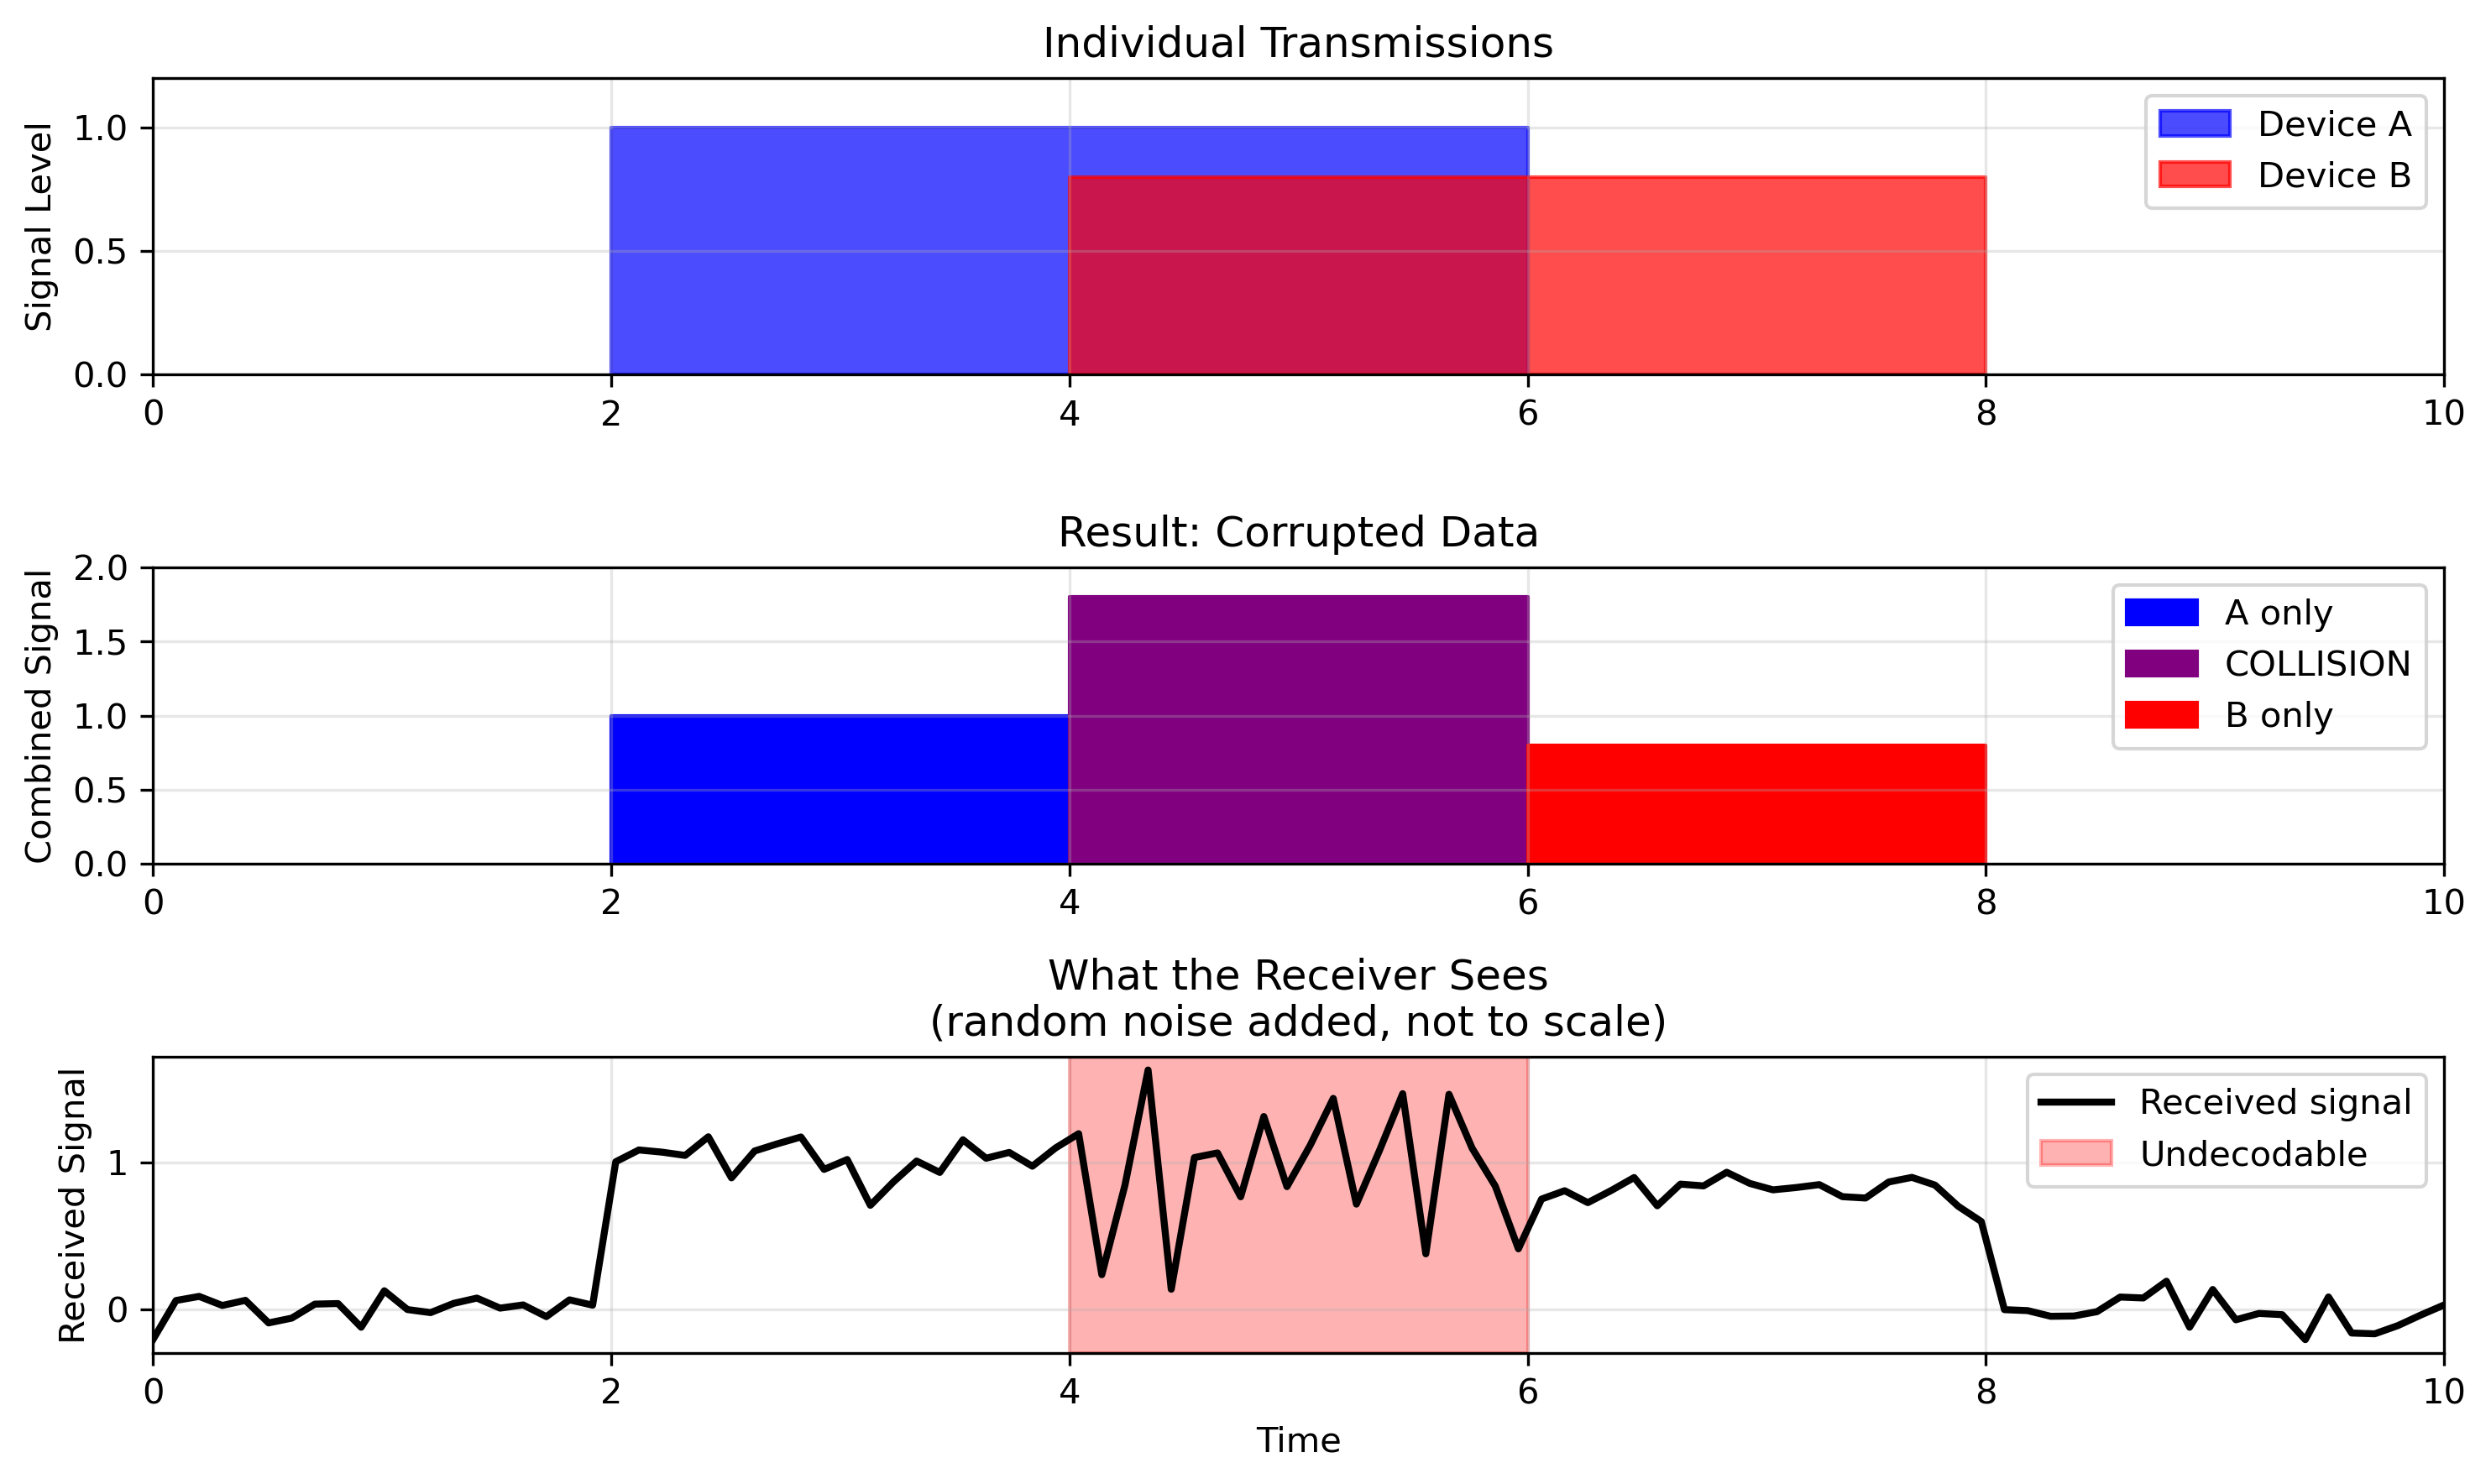
\includegraphics[width=\textwidth]{assets/diagrams/csma/collisions.png}
    \caption{Example of a collision}
    \label{fig:collision_visualization}
\end{figure}

\newpage
\subsection{Carrier Sense Multiple Access (CSMA)}
Now that we understand the problem, let's understand one of the solutions.

CSMA works on a simple principle: before transmitting anything, a device listens to the channel to see if anyone else is already talking (carrier sensing). If the channel is free, it goes ahead and transmits. If someone else is already using the channel, it waits for its turn (busy waiting).

\begin{figure}[h]
    \centering
    \scalebox{0.7}{\input{assets/diagrams/csma/normal.latex}}
    \caption{CSMA Flowchart}
    \label{fig:csma-normal}
\end{figure}

\subsubsection{+ Collision Detection (CSMA/CD)}
CSMA/CD introduces real-time collision detection. The only difference from the barebones version is that while transmitting, devices continue listening to the channel. If they detect that their signal has been corrupted by interference (collision), they immediately stop transmitting and implement a "backoff" strategy.

The backoff algorithm uses exponential backoff, meaning that after multiple failed attempts, devices wait progressively longer before retrying. This prevents starvation\footnote{
    Starvation is a scheduling problem where a process is perpetually denied the resources it needs to proceed, often due to other processes monopolizing those resources or the algorithm causeing it to wait indefinitely.
}.
\subsubsection{+ Collision Avoidance (CSMA/CA)}
As the name implies, CSMA/CA tries to avoid colissions entirely.

The protocol uses a handshake mechanism called RTS/CTS (Request to Send/Clear to Send).

\speechleft{Device A}{"May I please transmit to Device C?" (RTS)}
\speechright{Device C}{"Yes, go ahead, I'm ready to listen" (CTS)}
\begin{tcolorbox}[colback=gray!10, colframe=gray!50, arc=3mm, left=2mm, right=2mm, boxrule=1pt, before skip=5mm, after skip=5mm]
    \textit{Other devices hear this exchange and know to stay quiet during the upcoming transmission}
\end{tcolorbox}
\speechleft{Device A}{\textit{Transmits data with confidence}}

You'll notice how prevalent this type of conversation (protocol design) is in networking. ACKs and NACKs and handshakes are everywhere! Network people have found that this approach works well and provides much needed structure to the communication process.

\subsection{Persistence}
You might also be wondering how long a device should wait before trying to transmit again after a collision or when the channel becomes free. I guarantee you that this is something you have already thought about, but this is just about putting a name to it. 


\subsubsection{1-Persistent CSMA}
In 1-persistent CSMA, when a device finds the channel busy, it continuously monitors the channel and transmits immediately when it becomes free. This is the most aggressive approach - devices are "persistent" with probability 1.

While this minimizes delay when the channel becomes available, it also maximizes the probability of collisions when multiple devices are waiting. If two or more devices are listening to a busy channel, they will all attempt to transmit simultaneously once it's free.

\subsubsection{Non-Persistent CSMA}
Non-persistent CSMA takes the opposite approach. When a device finds the channel busy, it waits for a random amount of time before checking again, rather than continuously monitoring.

This reduces the collision probability since devices don't all rush to transmit at the exact moment the channel becomes free. However, it can lead to wasted channel capacity - the channel might sit idle while devices are in their random wait periods.

\subsubsection{p-Persistent CSMA}
p-persistent CSMA offers a compromise between the two extremes. When the channel becomes free, each device transmits with probability \textit{p}, or waits until the next time slot with probability \textit{(1-p)}.

The value of \textit{p} can be tuned based on network conditions - lower values reduce collisions but increase delay, while higher values do the opposite. This approach is commonly used in slotted networks where time is divided into discrete slots.

% /assets/osi/datalink/csma/persistence.png
\begin{figure}[h]
    \centering
    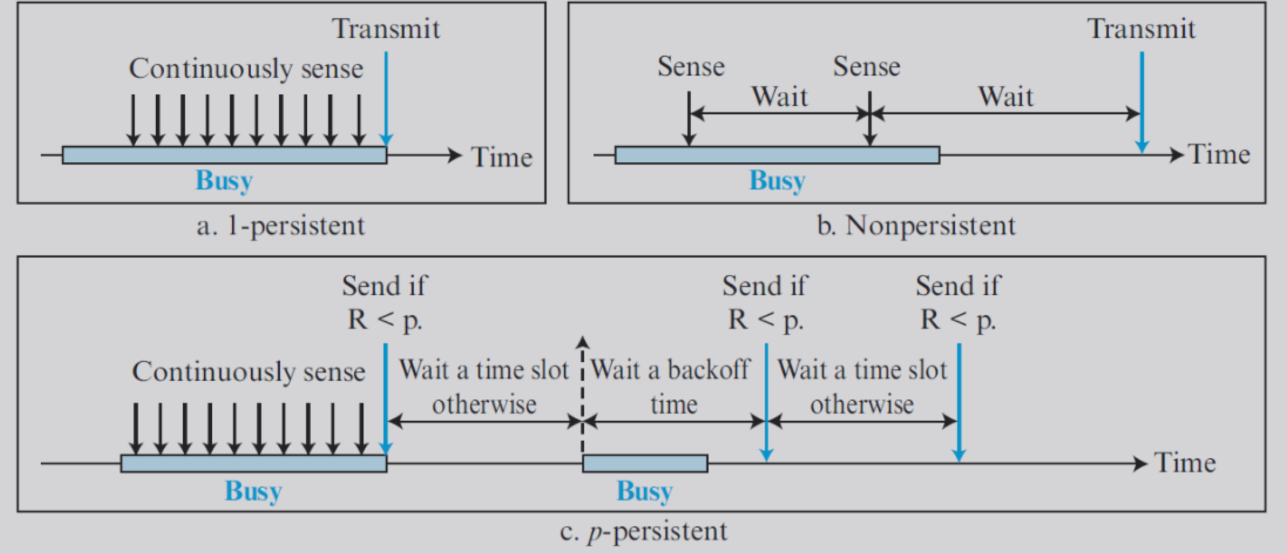
\includegraphics[width=.8\textwidth]{assets/osi/datalink/csma/persistence.png}
    \caption{Persistence in CSMA}
    \label{fig:csma-persistence}
\end{figure}